\newcommand{\D}{D}
\chapter{\D}

For the purposes of describing size-change termination we'll consider a language
\mono{D}. The following chapter describes the syntax and semantics of the
language.

\section{General properties}

The intent of the language is for it be used to explain concepts such as
size-change termination. One of the fundamental concepts required of the
language of application is that it's datatypes are well-founded. That is, any
subset $S$ of the range of values of some well-defined type has a value $s$
s.t. $\forall {s'\in S}\ s\leq s'$. This makes it ideal to chose some
oversimplistic data type structure rather than an army of basic types. Besides,
an apropriately defined basic data type should be able to represent arbitrarily
complex data values.

The language is initially first-order since the size-change termination
principle is first described for first-order programs later on in this work.
However, the language is designed so that it is easy to turn it into a
high-level language without much effort. This may prove necessary as we try to
expand size-change termination to higher-order programs.

The language is a call-by-value and purely functional to avoid any problems
that could arise from regarding lazy programs or where the notion of a global
state of the machine is relevant. Simply put, this is done to ensure elegance
of further proof with the help of the language.


\section{Data}

\D{} is a simple language where the emphasis is on the sizes of data. Hence,
the way that data values are constructed does not have to be particularly
practical, but all values have to be well founded and easily comparable.

The language \D{} is untyped, and represents all data in terms of
\emph{unlabeled ordered binary trees}, henceforth referred to as simply,
\emph{binary trees}. Such a tree is recursively defined as follows:

\begin{definition}

A binary tree is a set that is either empty, heneceforth refferred to as leaf,
or contains a single unlabeled node with two binary trees as it's left and
right child, henceforth simply reffered to as node. We'll refer to the set of
all possible values in \D{} as $\mathbb{B}$.

\end{definition}

To operate on such trees we'll require a few primitives, namely a
representation of leafs, recursive construction and destruction of nodes, as
well as a way to tell nodes and leafs apart. Most of these will be derived in
the operational semantics of \D{}\footnote{See \referToSection{d-sos}.},
however, we do require the following basic definitions:

\begin{definition}

Let the atom $0$ represent a leaf binary tree.

\end{definition}

\begin{definition}

The function $\cdot
:\mathbb{B}\times\mathbb{B}\rightarrow\mathbb{B}$ constructs a node with the
two arguments as it's left and right child, respectively. 

\end{definition}


\section{Syntax}\label{section:d-syntax}

We describe the syntax of \D in terms of an extended Backus-Naur
form\footnote{The extension lends some constructs from regular expressions to
achieve a more concise dialect. The extension is described in detail in
\referToAppendix{ebnf}.}. This is a core syntax definition, and other, more
practical, syntactical features may be defined later on as needed.

\begin{align}
\nonterm{expression}\ ::=&\ \nonterm{value}\ (\ \term{.}\ \nonterm{expression}
\ )\ ?\\
\nonterm{value}\ ::=&\ \term{0}\ |\ \term{(}\ \nonterm{value}\ \term{)}\ |
\ \nonterm{application}\\
\nonterm{application}\ ::=&\ \nonterm{name}
\ \nonterm{expression}^*\\
\nonterm{function}\ ::=&\ \nonterm{name}\ \nonterm{pattern}^*
\ \term{:=}\ \nonterm{expression}\\
\nonterm{pattern}\ ::=&\ \nonterm{pattern-value}\ (\ \term{.}
\ \nonterm{pattern}\ )\ ?\\
\nonterm{pattern-value}\ ::=&\ \term{0}\ |\ \term{\_}\ |\ \term{(}
\ \nonterm{pattern}\ \term{)}\ |\ \nonterm{name}\\
\nonterm{name}\ ::=&\ [\term{a}\mathmono{-}\term{z}]
\ \left (\ [\term{-}\ \term{a}\mathmono{-}\term{z}]^*
\ [\term{a}\mathmono{-}\term{z}]\ \right )?
\end{align}

The term $\term{\_}$ in $\nonterm{pattern-value}$ is the conventional wildcard
operator; it indicates a value that won't used by the function declaration, but
allows us to keep the same function signature. We define the \emph{signature}
of a function as follows:

\begin{definition}

A function signature in D consists of the function name and the number of
parameters it has.

\end{definition}

% TODO this should be clear from the semantics.

% Multiple wildcards in the parameter list indicate possibly different value
% arguments, while multiple occurances of the same variable name in the parameter
% list are disallowed.

\section{Semantics}\label{section:d-sos}

% Revise the context of an expression within a function call, it should always be
% the context upon entering the function call! Or even better, the context when
% the function was defined!

% \textbf{Allow mutual recursion}

% \textbf{Perhaps pattern matching must be exhaustive in general.}

% \textbf{Every subsequent definition must be strictly less specific than the former.}

In the following section we describe the semantics of \D{} using a form of
structured operational semantics. The syntax used to define the reduction rules
is largely equivalent to the Aarhus report\cite{sos}, but differs
slightly\footnote{The syntax applied here is described in further detail in
\referToAppendix{sos}.}.

\subsection{The memory model}\label{section:d-semantics-memory}

\begin{definition}\label{definition:memory} Memory is considered in terms of a
binary relation $\sigma$ which for any given clause $c$ is the set $\{(n,b)\mid
n\in\mathbb{N} \wedge b\in\mathbb{B} \wedge n\in P_c\}$. For any given
$(n,b)\in\sigma_c$, we say that in the scope of $c$, the variable $n$, is bound
to $b$.\end{definition}

\begin{corollary}\label{corollary:init-empty-scope} Variables are bound when
arguments are matched to clause patterns, and if the argument matches a
pattern, hence before pattern matching the arguments for any given clause $c$,
$\sigma_c=\emptyset$.\end{corollary}

\referToDefinition{memory} and \referToCorollary{init-empty-scope} indicate
that \D{} is statically scoped.  Furthermore, \referToDefinition{memory} may
prove hampering if we were ever to extend \D{} with lambda calculus, but there
are initially no plans to do so.

\begin{definition} The \nonterm{expression} at the end of \nonterm{program} can
be considered as the main clause of a program, which we'll refer to as
$c_{main}$.\end{definition}

\begin{corollary} $\sigma_{c_{main}}=\emptyset$. \end{corollary}

% This renders $\sigma$ countably infinite since $\mathbb{V}$ is countably
% infinite.

\subsubsection{Functions and variables}

Due to \D{} being a first-order language, we should make sure to separate the
function and variable spaces. We'll represent these by $\phi$ and $\gamma$,
respectively.

Whenever we use $\sigma$, $\phi$ or $\gamma$ in set notation, we imply the sets
of the names of functions and variables, and not the stacks themselves
corresponding to those names.  Hence, $\sigma=\phi\cup\gamma$, and to keep \D{}
first-order we add the limitation that $\phi\cap\gamma=\emptyset$.

\subsubsection{Making \D{} higher order}

The only change that this would require is to let $\phi=\gamma=\sigma$.

\subsection{Function declarations}

Assuming that as a part of the semantic analysis all $\nonterm{declaration}$ with the same name are grouped into the set $\left\langle n F\right\rangle$

A declaration with a name $n$, a \emph{non-empty} pattern
list $P$ and an expression $e$ is stored in the function space $\phi$:

\begin{equation}\label{sem:declaration}
{\displaystyle
  \left\langle \phi(n)\mapsto \left\langle P, x, \phi\right\rangle\right\rangle
  \rightarrow
  \phi'
\over\displaystyle
  \left\langle n, P, x, \phi\right\rangle
  \rightarrow
  \phi'
}
\end{equation}

\subsection{Expression evaluation}

An expression $x$ is either the element $e$, or a construction of an element
$e_1$ with another expression $x_1$. That is, the binary infix operator $\cdot$
is right-associative, and has the following operational semantics:

\everymath{\displaystyle}

\begin{equation}
{\displaystyle
  \left\langle \proc{Single}, x,\sigma\right\rangle
  \rightarrow
  \left\langle v,\sigma\right\rangle
\vee
  \left\langle \proc{Chain}, x,\sigma\right\rangle
  \rightarrow
  \left\langle v,\sigma\right\rangle
\over\displaystyle
  \left\langle x,\sigma\right\rangle
  \rightarrow
  \left\langle v,\sigma\right\rangle
}
\end{equation}

\begin{equation}
{\displaystyle
  x\rightarrow e
\wedge
  \left\langle e,\sigma\right\rangle
  \rightarrow
  \left\langle v,\sigma\right\rangle
\over\displaystyle
  \left\langle \proc{Single}, x,\sigma\right\rangle
  \rightarrow
  \left\langle v,\sigma\right\rangle
}
\end{equation}

\begin{equation}
{\displaystyle
  x\Rightarrow e_1\cdot x_1
\wedge
  \left\langle e_1,\sigma\right\rangle
  \rightarrow
  \left\langle v_1,\sigma\right\rangle
\wedge
  \left\langle x_1,\sigma\right\rangle
  \rightarrow
  \left\langle v_2,\sigma\right\rangle
\over\displaystyle
  \left\langle \proc{Chain}, x, \sigma\right\rangle
  \rightarrow
  \left\langle v, \sigma\right\rangle
}
\quad(\text{where }v_1\cdot v_2=v)
\end{equation}

\subsection{Element evaluation}

According to the syntax specification, an element of an expression can either
be the atom $0$, or an application. We'd like to distinguish between variables
and functions, and we do that  

\begin{equation}
{\displaystyle
\left(
    e\Rightarrow 0
  \wedge
    v\equiv 0
\right)
\vee
{\displaystyle
    e\Rightarrow n
\over\displaystyle
    \beta(n)\Rightarrow v
}
\vee
{\displaystyle
    e\Rightarrow \left\langle n, X\right\rangle
\over\displaystyle
    \left\langle n,X,\sigma\right\rangle
    \Rightarrow
    \left\langle v,\sigma\right\rangle
}
\over\displaystyle
\left\langle e,\sigma\right\rangle
\Rightarrow
\left\langle v,\sigma\right\rangle
}
\end{equation}

\subsection{Function application}

\begin{equation}
{\displaystyle
{\displaystyle
{\displaystyle
  \left\langle n, \phi\right\rangle
  \Rightarrow
  \left\langle P, x, \phi\right\rangle
\over\displaystyle
  \left\langle P, X, \sigma\right\rangle
  \Rightarrow
  \sigma'
}
\over\displaystyle
  \left\langle x, \sigma'\right\rangle
  \Rightarrow
  \left\langle v,\sigma'\right\rangle
}
\over\displaystyle
    \left\langle n,X,\sigma\right\rangle
    \Rightarrow
    \left\langle v,\sigma\right\rangle
}
\end{equation}

\subsection{Pattern matching}

\begin{equation}
{\displaystyle
{\displaystyle
  \left\langle P_{head}, X_{head}, \sigma\right\rangle
  \Rightarrow
  \sigma''
\over\displaystyle
  \left\langle P_{tail}, X_{tail}, \sigma''\right\rangle
  \Rightarrow
  \sigma'
}
\over\displaystyle
  \left\langle P, X, \sigma\right\rangle
  \Rightarrow
  \sigma'
}
\end{equation}

\begin{equation}
{
  \left\langle\proc{I}, p,x,\sigma\right\rangle
  \Rightarrow
  \left\langle p',x',\sigma'\right\rangle
\vee
  \left\langle\proc{Z}, p,x,\sigma\right\rangle
  \Rightarrow
  \left\langle p',x',\sigma'\right\rangle
\vee
  \left\langle\proc{N}, p,x,\sigma\right\rangle
  \Rightarrow
  \left\langle p',x',\sigma'\right\rangle
\vee
  \left\langle\proc{P}, p,x,\sigma\right\rangle
  \Rightarrow
  \left\langle p',x',\sigma'\right\rangle
}\over{
  \left\langle p, x, \sigma\right\rangle
  \Rightarrow
  \left\langle p', x', \sigma'\right\rangle
}
\end{equation}

For the sake of an elegant notation, we'll override the function $\cdot$ for
patterns.

\begin{definition}

A pattern is an unlabeled of binary tree which is either empty or consists of
an unlabeled node with a $0$, $\_$, name, or a pattern as it's left and right
child. 

\end{definition}

\begin{definition}

Let the set of all possible patterns be denoted by $\mathbb{P}$.

\end{definition}

\begin{definition}

The function $\cdot
:\mathbb{P}\times\mathbb{P}\rightarrow\mathbb{P}$ constructs a pattern node with the
two arguments as it's left and right child, respectively. 

\end{definition}

\begin{equation}
{
    p\Rightarrow \_\cdot p'
  \wedge
    x\Rightarrow e\cdot x'
  \wedge
    \sigma\Rightarrow\sigma'
}\over{
  \left\langle\proc{Underscore}, p,x,\sigma\right\rangle
  \Rightarrow
  \left\langle p',x',\sigma'\right\rangle
}
\end{equation}

\begin{equation}
{
    p\Rightarrow 0\cdot p'
  \wedge
    x\Rightarrow e\cdot x'
  \wedge
    \sigma\Rightarrow\sigma'
}\over{
  \left\langle\proc{Zero}, p,x,\sigma\right\rangle
  \Rightarrow
  \left\langle p',x',\sigma'\right\rangle
}
\end{equation}


\begin{equation}
{\displaystyle
{\displaystyle
{\displaystyle
    p\Rightarrow n\cdot p'
  \wedge
    x\Rightarrow e\cdot x'
\over\displaystyle
    \left\langle e,\sigma\right\rangle
    \Rightarrow
    \left\langle v,\sigma\right\rangle
}\over\displaystyle
    \left\langle\sigma(n)\leftarrow v\right\rangle
    \Rightarrow
    \sigma'
}\over\displaystyle
  \left\langle\proc{Name}, p,x,\sigma\right\rangle
  \Rightarrow
  \left\langle p',x',\sigma'\right\rangle
}
\end{equation}

\begin{equation}
{\displaystyle
{\displaystyle
    p\Rightarrow p''\cdot p'  
  \wedge
    x\Rightarrow x''\cdot x'
\over\displaystyle
  \left\langle p'', x'', \sigma\right\rangle
  \Rightarrow
  \sigma'
}
\over\displaystyle
  \left\langle\proc{Pattern}, p,x,\sigma\right\rangle
  \Rightarrow
  \left\langle p',x',\sigma'\right\rangle
}
\end{equation}

\subsection{Deducing unary functions from multivariate functions}

When performing termination analysis of programs it may prove tedious to
consider a list of patterns rather than a single pattern, especially since a
multivariate function can always be encoded as a unary function with e.g. the
patterns \mono{a}, \mono{b}, \mono{c}, and d encoded as \mono{a.b.c.d}. The
same ``encoding'' would have to be applied to each call to the function as
well. Hence, we can limit ourselves to termination proofs of unary functions.

\input{language/input}
\section{Size}

For the purposes of talking about size-change termination, we also need to
define the notion of size, and be sure to do so in such a way so that all
possible data values are well-founded.

\begin{definition}\label{definition:size}

Size of a value in \D{} is the number of nodes in the tree representing
that value.

\end{definition}

The ``well-foundedness'' of \D{}'s data values, given such a definition can be
argued for by proving a bijective relation between $\mathbb{B}$ and
$\mathbb{N}$. This would imply that we can define the relation $<$ on \D{}'s
data values, which we know to be well-founded.

We start by formally proving that \referToDefinition{size} yields a many-to-one
mapping of \D{}'s data values to the natural numbers.

First, we prove, by induction, that any natural number can be represented in
\D{}:

\begin{proof}\ \\

\begin{description}[\setleftmargin{70pt}\setlabelstyle{\bf}]

\item [Base] The atom $0$ has no nodes, and hence represents the value $0$.

\item [Assumption] If we can represent the $n\in\mathbb{N}$ in \D{}, then
we can also represent the number $n+1\in\mathbb{N}$. 

\item [Induction] Let $n$ be represented by some binary tree $A$, then $n+1$
can be represented by $0\cdot A$. 

\end{description}

\end{proof}

Second, we prove, also by induction, that any value in \D{} has one and only
one representation in $\mathbb{N}$.

\begin{proof}\ \\

\begin{description}[\setleftmargin{70pt}\setlabelstyle{\bf}]

\item [Base] The atom $0$ has no nodes, and hence corresponds only to the value
$0$.

\item [Assumption]

\begin{enumerate}

\item If the binary tree $A$ has only one representation $n\in\mathbb{N}$, then
$\left|0\cdot A\right|\equiv n+1$ and $\left|A\cdot 0\right|\equiv n+1$.

\item If the binary tree $A$ has only one representation $n\in\mathbb{N}$, and
the binary tree $B$ has only one representation $m\in\mathbb{N}$, then
$\left|A\cdot B\right|\equiv n+m+1$ and $\left|B\cdot A\right|\equiv n+m+1$.

\end{enumerate}

\item [Induction]

By definition of the binary function $\cdot$, any given node $A$ with left
child $A_{left}$ and right child $A_{right}$ has the size:

$$\left|A\right|=1+\left|A_{left}\right|+\left|A_{right}\right|$$

Hence, any value in \D{} must have one and only one representation in
$\mathbb{N}$.

\end{description}

\end{proof}

\referToDefinition{size} \emph{almost} allows us to devise an algorithm to
compare the sizes of data values. The problem withstanding is that two
different values can have rather diverging tree representations. Hence,
comparing them, using only the operations defined in \referToSection{d-sos}, is
seemingly impossible unless we initially, or along the way, transform the
binary trees being compared into some sort of a \emph{standard representation}.
We'll define this representation, recursively, as follows:

\begin{definition}\label{definition:standard-representation}

A binary tree in standard representation is a binary tree that either is a leaf
or a node having a leaf as its left child and a binary tree in standard
representation as its right child.

\end{definition}

Intuitively, a binary tree in standard representation is just a tree that only
descends along the right side. Comparing the sizes of two trees in this
representation is just a matter of walking the descending in the two trees
simultaneously, until one of them, or both, bottom out. If there is a tree that
bottoms out strictly before another, that is the lesser tree by
\referToDefinition{size}. \referToFigure{standard-representation} showcases
some examples.

\begin{figure}[htbp!]
\centering
\subfigure[{Not in standard representation}]
{
  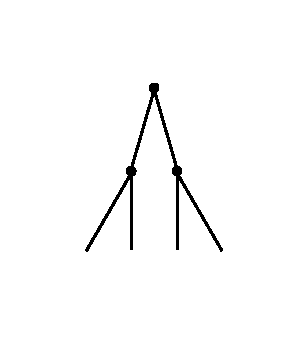
\includegraphics[scale=1]{figures/first-non-standard}
}
\subfigure[{Not in standard representation}]
{
  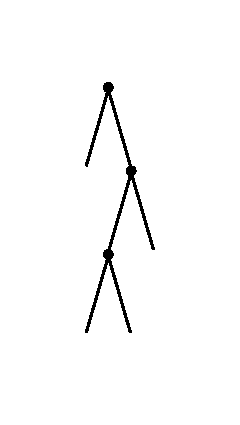
\includegraphics[scale=1]{figures/second-non-standard}
}
\subfigure[{Standard representation}]
{
  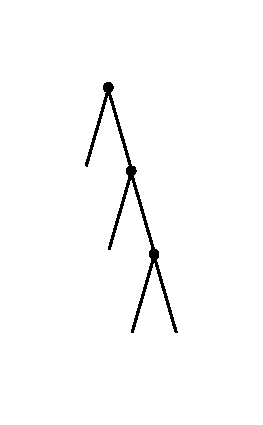
\includegraphics[scale=1]{figures/standard}
}
\caption[]{Three trees of various shapes but equal size.}
\label{figure:standard-representation}
\end{figure}

\subsection{\mono{normalize/1}}

\begin{verbatim}
normalize a = normalize-aux a 0 0

normalize-aux 0     0     an = an
normalize-aux 0     bl.br an = normalize-aux bl br    an
normalize-aux 0.ar  b     an = normalize-aux ar b     0.an
normalize-aux al.0  b     an = normalize-aux al b     0.an
normalize-aux al.ar b     an = normalize-aux ar al.b  0.an

\end{verbatim}

\subsubsection{Correctness}

\mono{normalize/1} makes use of an auxiliary procedure, \mono{normalize-aux/3},
for which we can provide the following argument descriptions:

\begin{enumerate}

\item The tree to be normalized.

\item An auxiliary tree.

\item A normalized tree.

\end{enumerate} 

The idea of the algorithm is to move right-wise down the tree to be normalized,
constructing an auxiliary tree containing all left-wise child nodes, if any.

The return value is the normalized tree, i.e. the third argument. Hence, we
must increase the size of the normalized tree each time we move right-wise down
the tree to be normalized.

Once we reach the right-most leaf of the tree to be normalized we return the
normalized tree if the auxiliary tree is empty. Otherwise, we normalize the
right child of the auxilary tree, with the left child of the auxiliary as the
new auxiliary tree, and the normalized tree constructed thus far as the initial
normalized tree.

\subsubsection{Time complexity}

Coming soon..

\subsubsection{Space complexity}

Coming soon..

\subsection{\mono{less/2}}\label{section:d-size-less}

We'll define the function \mono{normalize/1} further below to transform any
\D{} value into its standard representation. For now we'll assume that we have
such a function in scope and define \mono{less/2} for determining whether the
value of the first argument is strictly less than the value of the second
argument.

In order to define such a boolean-valued function we need a convention for
representing the boolean values $true$ and $false$ in \D{}. We'll adopt the
C-like convention:

\begin{definition}

A $false$ value is represented by a leaf tree. A $true$ value is represented by
a non-leaf tree, i.e. a node.

\end{definition}

We're now ready to define the function \mono{less/2}:

\begin{lstlisting}[label={listing:d-less},caption={A definition of the \mono{less/2} function.}]
less a b := normalized-less (normalize a) (normalize b)

normalized-less 0 b := b
normalized-less _ 0 := 0
normalized-less _.a _.b := normalized-less a b
\end{lstlisting}

\subsubsection{Correctness}

\begin{proof}

Given \referToDefinition{standard-representation}, and the assumption that
$\proc{Normalize}(A)$ computes the standard representation of $A$, we know the
following:

\begin{enumerate}

\item $\left|A\right|\equiv\left|\proc{Normalize}(A)\right|$.

\item We'll walk through all the nodes if we perform a recursive
right-child-walk starting at $A$.

\item The same holds for $B$.

\end{enumerate}

It is also easy to see from lines
\ref{normalized-less-init-start}:\ref{normalized-less-init-end} that
$\proc{NormalizedLess}$ stops as soon as we reach the ``bottom'' of either $A$
or $B$.

Given \referToDefinition{size}, $A<B$ iff it bottoms out before $B$, that is,
we reach an instance of the recursion where both $IsLeaf(A)$ and $IsNode(B)$
hold.  In all other cases $A\geq B$, the cases specifically are:

\begin{itemize}

\item $IsLeaf(A)$ and $IsLeaf(B)$, then $\left|A\right|\equiv \left|B\right|$.

\item $IsNode(A)$ and $IsLeaf(B)$, then $\left|A\right|>\left|B\right|$

\end{itemize}

Last but not least, due to all data values being finite, eventually one of the
trees does bottom out.

\end{proof}

\subsubsection{Time complexity}

Given that the binary trees $A$ and $B$ are in standard representation when we
enter the auxiliary procedure, $\proc{NormalizedLess}$, it is fairly easy to
get an upper bound on the running time of $\proc{NormalizedLess}$ itself.

Indeed, the running time of $\proc{NormalizedLess}$ itself is
$O\left(\proc{Max}\left(\left|A\right|,\left|B\right|\right)\right)$, since we
just walk down the trees until one of them bottoms out. 

We haven't yet defined the procedure $\proc{Normalize}$ yet. Hence, the only
thing that we can say about the running time of $\proc{Less}$ in general is
that it is $O\left(\proc{Normalize}(A) + \proc{Normalize}(B) +
\proc{Max}\left(\left|A\right|,\left|B\right|\right) \right)$.

\subsubsection{Space complexity}

Coming soon..

\subsection{Built-in high-order
functions}\label{section:language-higher-order-built-ins}

Although \mono{D} is initially a first-order language, we will ignore that
limitation for a bit and define a few higher-order functions to provide some
syntactical sugar to the language. Beyond the discussion in this section, these
higher-order functions should be regarded as \mono{D} built-ins.

\subsubsection{Branching}

In the following definition, the variable names \mono{true} and \mono{false}
refer to expressions to be executed in either case.

\begin{verbatim}
if 0 _ false := false
if _._ _ true := true
\end{verbatim}

As you can see, we employ the C convention that any value other than $0$ is a
``truthy'' value, and the expression \mono{true} is returned.

Although the call-by-value nature of the language does not allow for
short-circuiting the if-statements defined in such a way, this shouldn't be any
impediment to further analysis.

\subsection{Sample programs}

As an illustration of the language syntax, the following program reverses a tree:

\begin{verbatim}
reverse 0 := 0
reverse left.right := (reverse right).(reverse left)
\end{verbatim}

The following program computes the Fibonacci number \mono{n}:

\begin{verbatim}
fibonacci 0 x y := 0
fibonacci 0.0 x y := y
fibonacci n x y := fibonacci (minus n 0.0) y (add x y)
\end{verbatim}

